\documentclass[letterpaper,9pt]{article}
\usepackage[utf8]{inputenc}
\usepackage{latexsym}
\usepackage[empty]{fullpage}
\usepackage{graphicx}
\usepackage{array}
\usepackage[left=2cm,right=2cm,top=2cm,bottom=2cm]{geometry}
\usepackage{titlesec}
\usepackage{marvosym}
\usepackage[usenames,dvipsnames]{color}
\usepackage{verbatim}
\usepackage{enumitem}
\usepackage{biblatex}
\addbibresource{sample.bib}
\usepackage{hyperref}
\hypersetup{
    colorlinks=true,
    linkcolor=blue,
    filecolor=magenta,      
    urlcolor=cyan,
} 
\urlstyle{same}
\usepackage{fancyhdr}

\pagestyle{fancy}
\fancyhf{} % clear all header and footer fields
\fancyfoot{}
\renewcommand{\headrulewidth}{0pt}
\renewcommand{\footrulewidth}{0pt}

% Adjust margins
\addtolength{\oddsidemargin}{-0.375in}
\addtolength{\evensidemargin}{-0.375in}
\addtolength{\textwidth}{1in}
\addtolength{\topmargin}{-0.5in}
\addtolength{\textheight}{1.0in}

\urlstyle{same}

\raggedbottom
\raggedright
\setlength{\tabcolsep}{0in}

% Sections formatting
\titleformat{\section}{
  \vspace{-4pt}\scshape\raggedright\large
}{}{0em}{}[\color{black}\titlerule \vspace{-5pt}]

%-------------------------
% Custom commands
\newcommand{\resumeItem}[2]{
  \item\small{
    {#1} { #2 \vspace{-2pt}}
  }
}

\newcommand{\resumeSubheading}[4]{
  \vspace{-1pt}\item
    \begin{tabular*}{0.97\textwidth}{l@{\extracolsep{\fill}}r}
      \textbf{#1} & #2 \\
      \textit{\small#3} & \textit{\small #4} \\
    \end{tabular*}\vspace{-5pt}
}

\newcommand{\resumeSubItem}[2]{\resumeItem{\textbf{#1}}{#2}\vspace{-4pt}}

\renewcommand{\labelitemii}{$\circ$}

\newcommand{\resumeSubHeadingListStart}{\begin{itemize}[leftmargin=*]}
\newcommand{\resumeSubHeadingListEnd}{\end{itemize}}
\newcommand{\resumeItemListStart}{\begin{itemize}}
\newcommand{\resumeItemListEnd}{\end{itemize}\vspace{-5pt}}

%-------------------------------------------
%%%%%%%%%%%  CV STARTS HERE  %%%%%%%%%%%%%%%%%%%%%%%%%%%%

\begin{document}

%----------HEADING-----------------
\begin{tabular}{ m{16cm} m{1cm} m{1cm} }
\begin{center}
\textbf{\LARGE KEDDOUCH LARBI}\\\

 \textbf{\large Ingénieur d'Etat en Systèmes Embarqués et Mobiles   }\\\
 
 ENSIAS, Avenue Mohamed Ben Abdellah Regragui, Rabat, Maroc |  +212 623255240 |
larbi.keddouch@um5s.net.ma | Nationalité : Marocain
\end{center}

   &  & \begin{flushright}
    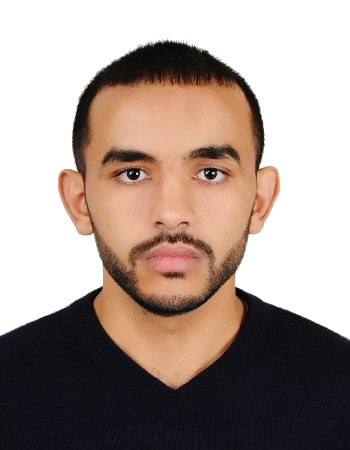
\includegraphics[scale=0.25]{image/Nekk.jpg}
    \end{flushright}  \\ 
\end{tabular} 



%-----------OBJECTIVE-----------------
%\section{ Objectif professionnel}
%Je cherche une opportunité de stage -projet de fin d'études- pour mettre mes connaissances académiques et expériences professionnelles en pratique, à fin de servir les objectifs de l'entreprise et élargir mes connaissances en Systèmes Embarqués. 
%-----------EDUCATION-----------------
\color{blue}
\section{Éducation \& Formation}
\color{black}
  \resumeSubHeadingListStart
    \resumeSubheading
      {École Nationale Supérieure d'Informatique et d'Analyse des Systèmes}{Rabat, Maroc}
      {Cycle d'ingénieur en Ingénierie des Systèmes Embarqués et Mobiles (ISEM)}{Septembre 2015 -- Septembre 2018}
    \resumeSubheading
      {Classes Préparatoires aux grandes écoles d'ingénieurs, Lycée mohamed reda slaoui}{Agadir, Maroc}
      {Filière: Technologies et Sciences Industrielles (TSI)}{Septembre 2012 -- Juin 2015}
    \resumeSubheading
    {Baccalauréat, Lycée Ibn Soulaimane Arrasmouki}{ Tiznit, Maroc}{Option: Sciences et Technologies Mécaniques (STM)}{Juin 2012}
  \resumeSubHeadingListEnd
\color{blue}
\section{Expérience}
\color{black}
%-----------EXPERIENCE-----------------
\resumeSubHeadingListStart
    \resumeSubheading
      {Foundation MASciR}{Madinat Al Irfane Rabat, Maroc}
      {Stage PFE}{Mars - Septembre 2018}
      \resumeItemListStart
        \resumeItem{réalisation d'un système de détection et d'identification dés non-conformités alimentaires dans le couscous pour la société Dari Couspate}{}
      	\resumeItem{Allègement d’un logiciel d'inspection visuelle développé au sein de l’équipe afin qu’il répond aux besoins du projet}{}
        \resumeItem{Algorithme de traitement d’image pour la détection des non-conformités}{}
        \resumeItem{Développement d’un dashboard pour l’affichage des résultats, statistiques et des données en temps réel}{}
        \resumeItem{Technologies utilisées: C++, Qt3.5, OpenCV, php, posgresql, Debian}{}
      \resumeItemListEnd
\resumeSubHeadingListEnd

\resumeSubHeadingListStart
    \resumeSubheading
      {INTELLCAP Group}{Agdal  Rabat, Maroc}
      {Stage technique}{Juillet - Septembre 2017}
      
      \resumeItemListStart
      \resumeItem{Développement d’un concept innovant d’un véhicule multi-missions de type UAV}{}
      \resumeItem{Technologies utilisées: Matlab, simulink, cycle de développement en V}{}
%        \resumeItem{Used the following technologies, tools and programming languages:}
%          {ASP.net, C\# , html , Visual Studio 2017 community and SQL Server Management Studio}
      \resumeItemListEnd
   
  \resumeSubHeadingListEnd

\resumeSubHeadingListStart
    \resumeSubheading
      {Ministere MFPMA}{Agdal  Rabat, Maroc}
      {Stage d'initiation}{Juillet - Septembre 2017}
      
      \resumeItemListStart
      	\resumeItem{Conception et réalisation d’une application de gestion des contacts du ministère}{}
        \resumeItem{Technologies utilisées: Visual studio, SQL server, C\#, ASP.NET, HTML, CSS }{}
%        \resumeItem{Used the following technologies, tools and programming languages:}
%          {ASP.net, C\# , html , Visual Studio 2017 community and SQL Server Management Studio}
      \resumeItemListEnd
   
  \resumeSubHeadingListEnd
 

%-----------PROJECTS-----------------
\color{blue}
\section{Projets}
\color{black}
  \resumeSubHeadingListStart
    \resumeSubItem
    {Développement d'une application de détection et de reconnaissance des plaques d'immatriculation}
      {} 
	\resumeItemListStart
		\resumeItem{Identification de la plaque d'immatriculation en utilisant les techniques de traitement d'image}{}
        \resumeItem{Reconnaissace de la plaque d'immatriculation en utilisant l'OCR}{}
        \resumeItem{Technologies utilisées: C++, OpenCV 3, Bibliotheque OCR, Visual studio, Linux Mint}{}
 	  %  \resumeItem{Use the following tools: Texas Instruments DSP TMS320C5x Evaluation Kit, Analog Discovery (Digilent EE Board), Acoustic acquisition board and Underwater Acoustic antennas}{}
      \resumeItemListEnd    
 %   \resumeSubItem
%    {Développement d'une application automobile de chauffage des sièges en utilisant les outils d'ArcCore et Matlab }{}
%    \resumeItemListStart
 %   	\resumeItem{Analyse du standard Autosar pour le Software automobile et simulation du prototype du système sur Simulink}{}
 %   	\resumeItem{Génération d'un fichier exécutable (.elf) à l'aide du core Autosar d'ArcCore pour la carte d'évaluation STM3210c }{}
 %   \resumeItemListEnd
    \resumeSubItem
    {Réalisation d’un système de reconnaissance faciale}{}
    \resumeItemListStart
    \resumeItem{Modéle de classification CNN: VGG16, AlexNet}{}
    \resumeItem{Intégration du modéle dans une application mobile android }{}
    \resumeItem{Technologies utilisées: Python, TensorFlow, Keras, Scikit-Learn, Android studio}{}
    \resumeItemListEnd
    \resumeSubItem
    {Développement d'une application desktop de gestion de formations au niveau des universités}
      {} 
	\resumeItemListStart
		\resumeItem{Gérer les formations, les formateurs et les étudiants au niveau de l'université}{}
        \resumeItem{Technologies utilisées: Langage C, Ubuntu}{}
 	  %  \resumeItem{Use the following tools: Texas Instruments DSP TMS320C5x Evaluation Kit, Analog Discovery (Digilent EE Board), Acoustic acquisition board and Underwater Acoustic antennas}{}
      \resumeItemListEnd    
    %\resumeSubItem
    %{Système de contrôle des feux de signalisation}
    %  {}
    %  \resumeItemListStart
    %    \resumeItem{Conception des blocks du système et implémentation en VHDL sur la carte de développement FPGA: Xilinx Spartan-3E}{}
    %  \resumeItemListEnd 
    
 \resumeSubItem
    {Projet système asservis: Smart home –SMART METER-}{}
    \resumeItemListStart
    \resumeItem{Technologies utilisées: capteurs, microcontroleur, android studio}{}
    \resumeItemListEnd    
    \resumeSubItem
    {Encore plus de projets sur mon profil Github: \url{https://github.com/larb1K3DD0UCH}}
      {}       
      \resumeSubHeadingListEnd
%
%--------PROGRAMMING SKILLS------------
\color{blue}
\section{Compétences}
\color{black}
 \resumeSubHeadingListStart
   \resumeSubItem{Langages de programmation et modélisation, Protocole de communication et réseaux}
      { : C/C++, Python, VHDL, langage assembleur, CAN, UART, SPI, Ethernet}
      \resumeSubItem{Environnement de développement integré et systèmes d'exploitation}{:LINUX(Ubuntu, Debian),  Visual Studio, Eclipse, Matlab/Octave, Xilinx ISE, PowerAMC, Netbeans IDE, Pycharm, Android
studio, Packet Tracer, Git (gestion de versions)}
      \resumeSubItem{Cartes de développement :}{  Arduino, STM32, raspberry pi 2, Xilinx Spartan-3E FPGA Starter Kit }
      \resumeSubItem{Outils d’analyse et de Conception :}{ Merise, UML, SysML, Modèle du cycle en V}
      \resumeSubItem{développement web :}{ ASP.NET, HTML, CSS}
      \resumeSubItem{Divers connaissances :}{ Machine Learning, Traitement d’image, Gestion des projets, Ingénierie des modèles, Cloud et virtualisation, recherche opérationnelle, probabilités et statistiques, management...}
      \resumeSubItem{Langues :}{ Tamazight (langue maternelle), Arabe(bilingue), Français (Courant) et Anglais(Courant)}
\resumeSubHeadingListEnd 

\color{blue}
\section{Certifications}
\color{black}
\resumeSubHeadingListStart
\resumeSubItem{Coursera}{Programmation Orienté Objet C++(ÉCOLE POLYTECHNIQUE FÉDÉRALE DE LAUSANNE)}
\resumeSubItem{Coursera}{Programming for Everybody (Getting Started with Python)}
\resumeSubItem{IBM}{Computer vision}
\resumeSubItem{IBM}{Intelligence artificielle}
\resumeSubHeadingListEnd 


\color{blue}
\section{Centres d'intérêt}
\color{black}
\resumeSubHeadingListStart
\resumeSubItem{}{Passionné par les nouvelles technologies}
\resumeSubItem{}{Sport(football, basketball)}
\resumeSubItem{}{Cinéma}
\resumeSubHeadingListEnd 


%-------------------------------------------
\end{document}
